\section{Units and Prefixes}
%By Matt Trawick

In this course, you are expected to know these standard prefixes to various units, and their abbreviations.  You'll especially be seeing a whole lot of nanoseconds (ns) and microns ($\mu$m).

\centerline{\hspace{0.5in}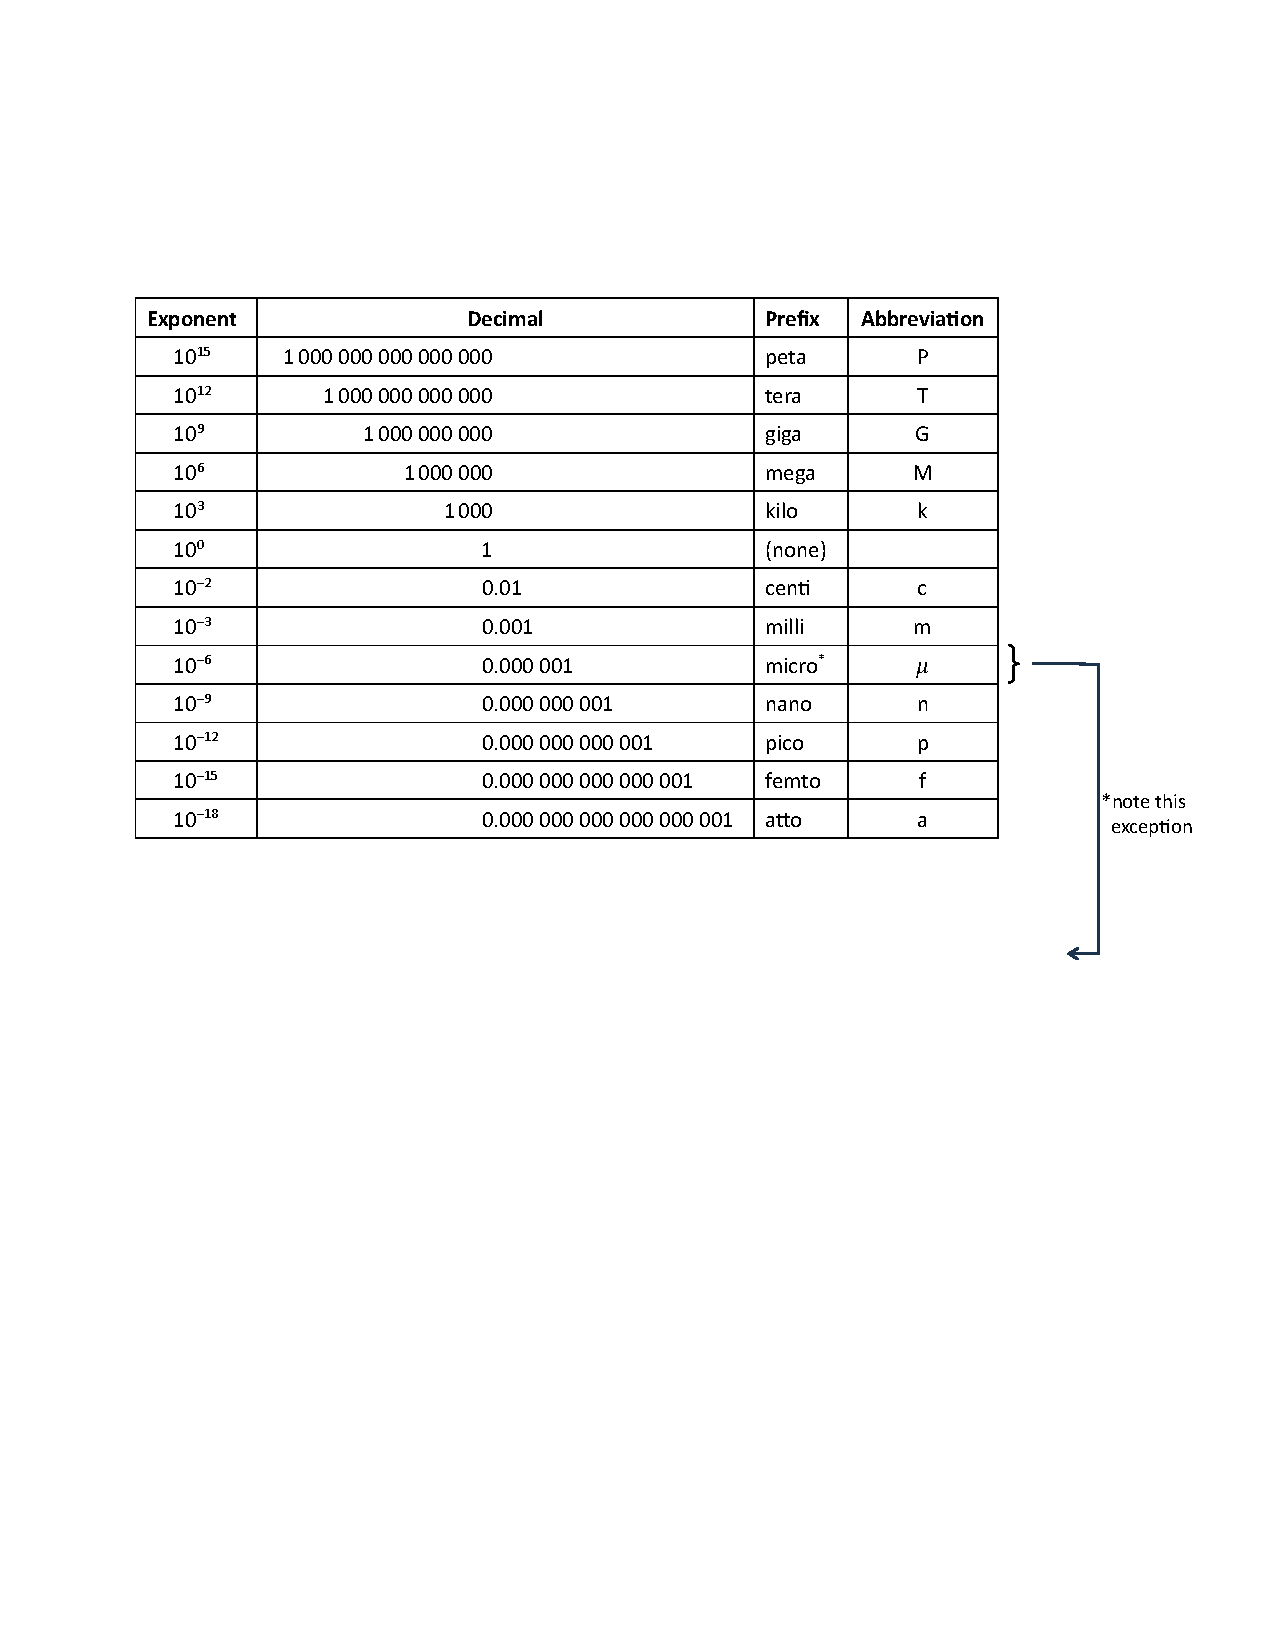
\includegraphics{appendices/si_prefixes.pdf}}

\vspace{-0.70in}
\textbf{Exceptions and other units:}

\begin{itemize}

\item \textbf{Microns:} The unit of $10^{-6}$ meters ($\mu$m) should logically be called a ``micrometer.''  In fact, it is\\
usually called a \textit{micron.}

\item \textbf{{\AA}ngstroms:} Historically, wavelengths of light are often measured in units of $10^{-10}$~meters, known as \AA ngstroms (abbreviation \AA), after the Swedish physicist Anders Jonas {\AA}ngstr\"{o}m.  A typical wavelength for red light could be written as either 650~nm or 6500~\AA.

\item \textbf{Light-years:} One light-year (abbreviation ly or l.y.) is the distance that light can travel in one year (in a vacuum), or about $9.46\times10^{15}$~meters.  The speed of light is thus one light-year per year, or 1~ly/y.

\item \textbf{Parsecs:} Often used by astronomers, one parsec (abbreviation pc) is roughly 3.26 light-years, or about $3.09\times10^{16}$ meters.\footnote{Hilariously, the original Star Wars movie in 1977 made a bad blunder involving parsecs when Han Solo claimed that his ship, the Millenium Falcon, ``made the Kessel Run in less than 12 parsecs.''  
This makes no sense, as the parsec is a unit of distance, not time.  In Han's defense, there is \textit{some} etymological connection between parsecs and seconds: astronomers use one \textit{arcminute} to mean 1/60 of a degree of angle, and one \textit{arcsecond} to mean 1/60 of an arcminute, or 1/3600 of a degree.  
The word parsec is a shortening of the phrase ``parallax of one arcsecond.'' The full meaning of that phrase is complicated, but ultimately one parsec is how far you would need to be from our Solar system for the distance between the Earth and the Sun (about 93~million miles) to be separated by exactly one arcsecond in your field of view.  (Fun facts, to know and share!)
}

\end{itemize}